\documentclass{article}
\usepackage{amsfonts,amssymb,amsmath,amsthm}

%% set-style letters
\def\AA{{\mathbb{A}}}
\def\BB{{\mathbb{B}}}
\def\CC{{\mathbb{C}}}
\def\DD{{\mathbb{D}}}
\def\EE{{\mathbb{E}}}
\def\FF{{\mathbb{F}}}
\def\GG{{\mathbb{G}}}
\def\HH{{\mathbb{H}}}
\def\II{{\mathbb{I}}}
\def\JJ{{\mathbb{J}}}
\def\KK{{\mathbb{K}}}
\def\LL{{\mathbb{L}}}
\def\MM{{\mathbb{M}}}
\def\NN{{\mathbb{N}}}
\def\OO{{\mathbb{O}}}
\def\PP{{\mathbb{P}}}
\def\QQ{{\mathbb{Q}}}
\def\RR{{\mathbb{R}}}
\def\SS{{\mathbb{S}}}
\def\TT{{\mathbb{T}}}
\def\UU{{\mathbb{U}}}
\def\VV{{\mathbb{V}}}
\def\WW{{\mathbb{W}}}
\def\XX{{\mathbb{X}}}
\def\YY{{\mathbb{Y}}}
\def\ZZ{{\mathbb{Z}}}

%% calligraphic letters
\def\cA{{\mathcal{A}}}
\def\cB{{\mathcal{B}}}
\def\cC{{\mathcal{C}}}
\def\cD{{\mathcal{D}}}
\def\cE{{\mathcal{E}}}
\def\cF{{\mathcal{F}}}
\def\cG{{\mathcal{G}}}
\def\cH{{\mathcal{H}}}
\def\cI{{\mathcal{I}}}
\def\cJ{{\mathcal{J}}}
\def\cK{{\mathcal{K}}}
\def\cL{{\mathcal{L}}}
\def\cM{{\mathcal{M}}}
\def\cN{{\mathcal{N}}}
\def\cO{{\mathcal{O}}}
\def\cP{{\mathcal{P}}}
\def\cQ{{\mathcal{Q}}}
\def\cR{{\mathcal{R}}}
\def\cS{{\mathcal{S}}}
\def\cT{{\mathcal{T}}}
\def\cU{{\mathcal{U}}}
\def\cV{{\mathcal{V}}}
\def\cW{{\mathcal{W}}}
\def\cX{{\mathcal{X}}}
\def\cY{{\mathcal{Y}}}
\def\cZ{{\mathcal{Z}}}
\def\cKL{{\mathcal{KL}}}

%% bold letters
\def\bA{{\bf{A}}}
\def\bB{{\bf{B}}}
\def\bC{{\bf{C}}}
\def\bD{{\bf{D}}}
\def\bE{{\bf{E}}}
\def\bF{{\bf{F}}}
\def\bG{{\bf{G}}}
\def\bH{{\bf{H}}}
\def\bI{{\bf{I}}}
\def\bJ{{\bf{J}}}
\def\bK{{\bf{K}}}
\def\bL{{\bf{L}}}
\def\bM{{\bf{M}}}
\def\bN{{\bf{N}}}
\def\bO{{\bf{O}}}
\def\bP{{\bf{P}}}
\def\bQ{{\bf{Q}}}
\def\bR{{\bf{R}}}
\def\bS{{\bf{S}}}
\def\bT{{\bf{T}}}
\def\bU{{\bf{U}}}
\def\bV{{\bf{V}}}
\def\bW{{\bf{W}}}
\def\bX{{\bf{X}}}
\def\bY{{\bf{Y}}}
\def\bZ{{\bf{Z}}}
\def\ba{{\bf{a}}}
\def\bb{{\bf{b}}}
\def\bc{{\bf{c}}}
\def\bd{{\bf{d}}}
\def\be{{\bf{e}}}
\def\boldf{{\bf{f}}} %different
\def\bg{{\bf{g}}}
\def\bh{{\bf{h}}}
\def\bi{{\bf{i}}}
\def\bj{{\bf{j}}}
\def\bk{{\bf{k}}}
\def\bl{{\bf{l}}}
\def\bm{{\bf{m}}}
\def\bn{{\bf{n}}}
\def\bo{{\bf{o}}}
\def\bp{{\bf{p}}}
\def\bq{{\bf{q}}}
\def\br{{\bf{r}}}
\def\bs{{\bf{s}}}
\def\bt{{\bf{t}}}
\def\bu{{\bf{u}}}
\def\bv{{\bf{v}}}
\def\bw{{\bf{w}}}
\def\bx{{\bf{x}}}
\def\by{{\bf{y}}}
\def\bz{{\bf{z}}}

%% other symbols
\DeclareMathOperator{\1}{\mathbf{1}}
\DeclareMathOperator{\0}{\mathbf{0}}
\DeclareMathOperator{\Id}{I}
\newcommand{\td}{\mathfrak{t}} % discrete-time 
\newcommand{\tr}{^\top}

%% operators
\DeclareMathOperator{\col}{col}
\DeclareMathOperator{\diag}{diag}
\DeclareMathOperator{\blkdiag}{blkdiag}
\DeclareMathOperator{\rank}{rank}
\DeclareMathOperator{\dis}{d}
\DeclareMathOperator{\sat}{sat} 
\DeclareMathOperator{\convhull}{\textbf{co}}
\DeclareMathOperator{\argmin}{argmin}
\DeclareMathOperator{\argmax}{argmax}
\DeclareMathOperator{\spec}{spec}
\def\He#1{\texttt{\rm{He}}\left\{{#1}\right\}}
\DeclareMathOperator{\trace}{tr}
\newcommand{\Imag}{\mathrm{Im}}

%% shortcuts
\newcommand{\norm}[1]{\lvert #1\rvert}
\newcommand{\wnorm}[2]{\lvert #1\rvert^2_{#2}}
\newcommand{\pderiv}[2]{\dfrac{\partial #1}{\partial #2}}
\newcommand{\pdef}[1]{\SS_{\succ0}^{#1}}
\newcommand\psemidef[1]{\SS_{\succeq0}^{#1}}
\newcommand{\bmx}[1]{\left[\begin{matrix}#1\end{matrix}\right]}
\newcommand{\pmx}[1]{\left(\begin{matrix}#1\end{matrix}\right)}
\newcommand{\smallpmat}[1]{\left(\begin{smallmatrix} #1 \end{smallmatrix} \right)}
\newcommand{\smallqmat}[1]{\left[\begin{smallmatrix} #1 \end{smallmatrix} \right]}
\newcommand{\overbar}[1]{\mkern 1.5mu\overline{\mkern-1.5mu#1\mkern-1.5mu}\mkern 1.5mu}
\renewcommand{\underbar}[1]{\mkern 1mu\underline{\mkern-1mu#1\mkern-1mu}\mkern 1mu}

\usepackage{hyperref}
\usepackage{graphicx}
\usepackage{float}

% SCRIPTS FOR DOUBLE AND SINGLE IMAGE

% \begin{figure}[H]
%     \centering
%     \begin{subfigure}{0.4\textwidth}
%     \includegraphics[width=\textwidth]{}
%     \caption{}
%     \label{}
%     \end{subfigure}
%     \hfill
%     \begin{subfigure}{0.55\textwidth}
%     \includegraphics[width=\textwidth]{}
%     \caption{}
%     \label{}
%     \end{subfigure}
%     \caption{}
%     \label{}
% \end{figure}

% \begin{figure}[H]
%     \centering
%     \includegraphics[width=0.65\textwidth]{}
%     \caption{}
%     \label{}
% \end{figure}

\usepackage[margin=54pt]{geometry}
\usepackage{biblatex}
\addbibresource{../biblio.bib}


\begin{document}

\date{}
\author{Marco Sterlini}

\title{Journal}
\maketitle

Ordered list of problems and steps taken to solve them, or at least to understand them better.

\section*{Initial works}

The first weeks were spent understanding the papers and the Matlab code given by Sophie (\cite{automatica}, \cite{css-paper}, \cite{data-driven}) regarding the application of ETM to the NN controller of a linearized and non linearized pendulum. The aim is to save as much computational load as possible by putting ETM in between the layers. Doing so it is possible to decide whether propagating the current layer output to the activation function. 
The main computational save will regard directly the application of the activation function that, being non-linear, is the most expensive operation in the network.
Some sum ups can be found in the folders \textit{"Automatica paper discussion", "Dynamic ETM intro discussion", "Sector conditions intro discussion"}.

\subsection*{Faulty application of global sector conditions}

I tried to apply directly the proposition of Sophie's notes to the system portrayed in \cite{css-paper}. Everything is documented in the notes \textit{"Faulty implementation of dynamic ETM report"} in \textit{"extra material"} folder.

\section*{Reproducing the results of the papers}

A first attempt into the implementation has been portrayed in Matlab and immediately after in Python. The most used modules were \texttt{cvxpy} as a framework for LMI resolution and \texttt{NumPy} for generic mathematical manipulation. 

\subsection*{Linear Inverted Pendulum}
The system used in \cite{css-paper} has been implemented in Python. The same weights used in the paper have been used to build up the NN controller. The main module exploited is \texttt{PyTorch}, the activation functions used are saturations. Tweaking the LMI conditions I was able to obtain the same results of the paper with the same basins of attraction.
The main concern about the approach followed in the paper regards the ETM mechanism design:
$$
  \hat{\omega}^{i}(k) = \begin{cases}
    \omega^{i}(k) & \text{if } f^{i}(\omega^{i}(k), \hat{\omega}^{i}(k-1), \hat{\omega}^{i-1}(k)) \geq 0\\
    \hat{\omega}^{i}(k-1) & \text{otherwise}  
  \end{cases}
$$
Where 
$$ 
f^{i}(\omega^{i}(k), \hat{\omega}^{i}(k-1), \hat{\omega}^{i-1}(k)) = ||\hat{\omega}^{i}(k-1) - \omega^{i}(k)||^{2}_{q^{i}_{\Delta}} - ||\omega^{i}(k) - \omega^{i}_*||^{2}_{q^{i}_{\omega}} - ||\hat{\omega}^{i-1}(k) - \omega^{i-1}_*||^{2}_{q^{i-1}_{\hat{\omega}}}
$$
The good thing about this function is the capability to stop early the computation and avoid computing the remaining layer if one doesn't trigger. However, this capability looses meaning when applied to a 2 layer NN controller. The bad point lies instead in the term $\omega^{i}(k) = sat(\nu^{i}(k))$ that is required at each layer verification. The need to compute this term, hence computing the activation function, makes the ETM useless if not for the cascade effect that remains good but not enough to be worth the computational load.

Nevertheless, I was able to reproduce the results for the static ETM, and I was able to extend the problem to a dynamic ETM inspired by the work of \cite{data-driven}.

\section*{Adding the conditions for dynamic ETM}
The main logic was to update the data used to compute the new input to the system only when necessary:
$$
  \pmx{\chi \\ s} = \begin{cases}
    \pmx{\omega\\ k} & \text{if the memory is updated}\\ 
    \pmx{\chi_{k-1} \\ s_{k-1}} & \text{otherwise}
  \end{cases}
$$

With the ETM mechanism described as follows:

\begin{equation} \label{ETM-mechanism}
s^{+} = \text{min}_{m \in \NN} \left\{ m \geq s + 1 | \psi(\omega_m, \chi) \geq \rho \eta_m \right\}
\end{equation}


And $\eta$ dynamic is defined as:

\begin{equation} \label{eta-dyn}
  \eta^{+} = (\rho + \lambda) \eta - \psi(\omega_m, \chi)
\end{equation}
  

This formulation ensures $\eta$ to be always positive and made it possible to consider it as a positive system like in \cite{positive-systems}. 
As a quick proof I can say that if the triggering condition $\psi$ is negative then the positiveness of $\eta$ is trivial. If instead $\psi$ is positive and $\psi \geq \rho \eta $

\section*{Problem in the extension to custom trained NN controllers}

\section*{Idea to use Samuele's results to address robustness of a NN controlled system with integrator in DT}

\section*{Development of new controllers}

\subsection*{Reinforcement learning approach}

\subsection*{Deep learning approach of LQR controller} 

\section*{Problems in the addition of system non-linearities} 

\subsection*{Progressive simplification of the problem to understand the issue}

\subsection*{1 layer saturation controller to linear pendulum}

It works by putting $\alpha = 1$

\subsection*{1 layer saturation controller to linear pendulum with integrator in the state}

It works by putting $\alpha = 1$

\subsection*{Attempt on handcrafting NN}
Considerations on it can be found in the last subsection of \textit{"Linear integrator 1 dimension case"}.
I am now trying to train a 3-layer NN with deep learning method on a K matrix found with LQR method and not pole placement. It will then be attempted to:
\begin{itemize}
  \item Find a LMI solution for the system with integrator and non-linearity for the 3 layer network. If it doesn't work simplify the problem and add complexity bit by bit
  \item Test the K gain from LQR method to non-linear system with and without saturation
  \item Find the LMI solution for the non-linear system with input saturation: $u = sat(K_{LQR} \cdot x)$
\end{itemize}

\subsection*{1 layer saturation controller to non-linear pendulum with integrator in the state}
The system under analysis is represented by the dynamic:

$$
m l^{2} \ddot{\theta} = m g l\ sin(\theta) - \mu \dot{\theta} + u
$$

That discretized becomes:

$$
  \begin{cases}
    \theta^{+} = \theta + \dot{\theta} \delta t\\
    \dot{\theta}^{+} = \dot{\theta} + \ddot{\theta} \delta t = \dot{\theta} + (\frac{g}{l} sin(\theta) - \frac{\mu}{m l^{2}} \dot{\theta}) \delta t + \frac{dt}{m l^{2} u} \\
    \eta^{+} = \eta + y = \eta + (\theta - r)
  \end{cases}
$$

I want to deal with the non-linearity in the form of $sin(\theta) - \theta$. In order to do so, I add and subtract the term $\frac{g}{l} \cdot dt \cdot \theta$ to $\dot{\theta}$ dynamics. Then by expressing $\phi(\theta) = sin(\theta) - \theta$ I can rewrite the overall dynamics as:

\begin{equation}
  \bmx{
    \theta^{+} \\
    \dot{\theta}^{+} \\
    \eta^{+}
  } = \bmx{
    1 & \delta t & 0 \\
    \frac{g \cdot dt}{l} & 1 - \frac{\mu \cdot dt}{m l^{2}} & 0 \\
    1 & 0 & 1
  } \bmx{
    \theta \\
    \dot{\theta} \\
    \eta
  } + \bmx{
    0 \\
    \frac{dt}{m l^{2}} \\
    0
  } u + \bmx{
    0 \\
    \frac{g \cdot dt}{l} \\
    0 
  } \phi 
\end{equation}

With more condensed notation:
$$
  x^{+} = A x + B u + C \phi
$$

The sector conditions on the saturation are the same of \cite{css-extended} adapted for the single saturation case:
$$
N = \bmx{
\begin{array}{c|c|c}
  0 & 1 & 0 \\
  \hline
  K & 0 & 0
\end{array}
}
$$

Each element is null except for $N_{u \omega} = 1$ and $N_{\nu x} = K$ so to have:
\begin{align*}
  \nu &= N_{\nu x} \cdot x + N_{\nu \omega} \cdot \omega + N_{\nu b} = K x\\
  u &= N_{ux} \cdot x + N_{u \omega} \cdot \omega + N_{u b} = \omega = sat(\nu)
\end{align*}

In the end the control input is $u = sat(\nu) = sat(K x)$

I consider a quadratic Lyapunov function $V = \tilde{x}\tr P \tilde{x}$ and I want to bound $\Delta V$ to be strictly negative.
Expressing $\tilde{x}_*^{+}$ in a compact way:

$$
  \tilde{x}^{+} = A x + B u + C \phi - A x_* - B u_* - C \phi_* = A \tilde{x} + B \tilde{u} + C \tilde{\phi}
$$

In this expression $\tilde{u}$ can be expressed with respect to $\omega$ and $x$:
$$
  \tilde{u} = N_{ux} x + N_{u \omega} + N_{ub} - N_{ux} x_* - N_{u \omega} \omega_* - N_{ub} = N_{ux} \tilde{x} + N_{u \omega} \tilde{\omega}
$$

I consider now the change of variables $\psi = \nu - \omega$ to make the problem compliant with the sector conditions used in \cite{css-extended}:

\begin{align*}
  \tilde{\nu} &= R N_{\nu x} \tilde{x} \\
  \tilde{u} &= N_{ux} \tilde{x} + N_{u \omega} (\tilde{\nu} - \tilde{\psi}) = N_{ux} \tilde{x} + N_{u \omega} R N_{\nu x} \tilde{x} - N_{u \omega} \tilde{\psi} = (N_{ux} + N_{u \omega} R N_{\nu x}) \tilde{x} - N_{u \omega} \tilde{\psi} = R_{\omega} \tilde{x} - N_{u \omega} \tilde{\psi} \\
  \tilde{x}^{+} &= (A + B R_{\omega}) \tilde{x} - B N_{u \omega} \tilde{\psi} + C \tilde{\phi} = \bar{A} \tilde{x} + \bar{B} \tilde{\psi} + C \tilde{\phi}
\end{align*}

With \begin{itemize}
  \item $R = \left( \Id - N_{\nu \omega} \right)^{-1}$
  \item $R_{\omega} = N_{ux} + N_{u \omega} R N_{\nu x}$
  \item $\bar{A} = A + B R_{\omega}$
  \item $\bar{B} = - B N_{u \omega}$
\end{itemize}

I can express then:

\begin{align} \label{matricione}
  \Delta V &= (\tilde{x}^{+})\tr P \tilde{x}^{+} - \tilde{x}\tr P \tilde{x} = \left( \bar{A} \tilde{x} + \bar{B} \tilde{\psi} + C \tilde{\phi} \right)\tr P \left( \bar{A} \tilde{x} + \bar{B} \tilde{\psi} + C \tilde{\phi} \right) - \tilde{x}\tr P \tilde{x} = \\
  &= \bmx{
    \tilde{x}\\
    \tilde{\psi}\\
    \tilde{\phi}
  }\tr \bmx{
    \bar{A}\tr P \bar{A} - P & \bar{A}\tr P \bar{B} & \bar{A}\tr P C \\
    \bar{B}\tr P \bar{A} & \bar{B}\tr P \bar{B} & \bar{B}\tr P C \\
    C\tr P \bar{A} & C\tr P \bar{B} & C\tr P C
  } \bmx{
    \tilde{x}\\
    \tilde{\psi}\\
    \tilde{\phi}
  }
\end{align}

I have to include now the sector conditions to deal with the non-linearity of the activation functions of the NN controller. In this particular case we deal with only one saturation function. Following the approach in \cite{css-extended} I can express the sector condition as:

$$
  \tilde{\psi}\tr T \left[ G \tilde{x} - \tilde{\nu} + \tilde{\psi} \right] \leq 0 \to \bmx{
    \tilde{x} \\
    \tilde{\psi} \\
    \tilde{\phi}
  }\tr \bmx{
    0 & 0 & 0 & 0 \\
    TG & -T & T & 0 \\
    0 & 0 & 0 & 0
  } \bmx{
    \tilde{x} \\
    \tilde{\psi} \\
    \tilde{\nu} \\
    \tilde{\phi}
  } \to \bmx{
    \tilde{x} \\
    \tilde{\psi} \\
    \tilde{\phi}
  }\tr \bmx{
    0 & 0 & 0 & 0 \\
    TG & -T & T & 0 \\
    0 & 0 & 0 & 0
  } \bmx{
    \Id & 0 & 0 \\
    R N_{\nu x} & \Id - R & 0 \\
    0 & \Id & 0  \\
    0 & 0 & \Id
  } \bmx{
    \tilde{x} \\
    \tilde{\psi} \\
    \tilde{\phi}
  }
$$

Having written $\tilde{\nu} = N_{\nu x} \tilde{x} + N_{\nu \omega} \tilde{\omega} = N_{\nu x} \tilde{x} + N_{\nu \omega} (\tilde{\nu} - \tilde{\psi}) \to (\Id - N_{\nu \omega}) \tilde{\nu} = N_{\nu x} \tilde{x} - N_{\nu \pi} \tilde{\psi} \to \tilde{\nu} = R N_{\nu x} \tilde{x} + (\Id - R) \tilde{\psi}$ 
Exploiting the condition $N_{\nu \omega} = \Id - R^{-1} \to -R N_{\nu \omega} = \Id - R$

I can rewrite the sector conditions as:

\begin{align*}
  \bmx{
    \tilde{x} \\
    \tilde{\psi} \\
    \tilde{\phi}
  }\tr M_{1} R_{\phi} \bmx{
    \tilde{x} \\
    \tilde{\psi} \\
    \tilde{\phi}
  } \leq 0
\end{align*}

Given their sign definiteness I can subtract the term to $\Delta V$ in order to impose a negative bound to the Lyapunov function derivative:

$$
  \Delta V \leq \Delta V - He \left\{\bmx{
    \tilde{x} \\
    \tilde{\psi} \\
    \tilde{\phi}
  } M_{1} R_{\phi} \bmx{
    \tilde{x} \\
    \tilde{\psi} \\
    \tilde{\phi}
  }\right\} < 0
$$

Finally, I include the sector condition for the non-linearity $\phi = sin(\theta) - \theta$. The sector used is the following that is valid for $\theta \in \left[ -\pi, \pi \right]$:

\begin{align*}
  & \bmx{
    \tilde{\theta} \\
    sin(\tilde{\theta}) - \tilde{\theta}
  }\tr \bmx{
    0 & -1 \\
    -1 & -2
  } \bmx{
    \tilde{\theta} \\
    sin(\tilde{\theta}) - \tilde{\theta}
  } \geq 0 \to \\
  & \to \bmx{
    \tilde{x} \\
    \tilde{\psi} \\
    \tilde{\phi}
  }\tr \bmx{
    1 & 0 & 0 & 0_{1 \times n_{\phi}} & 0 \\
    & 0_{1 \times n_{x}} & & 0_{1 \times n_{\phi}} & 1
  }\tr \bmx{
    0 & -1 \\
    -1 & -2
  } \bmx{
    1 & 0 & 0 & 0_{1 \times n_{\phi}} & 0 \\
    & 0_{1 \times n_{x}} & & 0_{1 \times n_{\phi}} & 1
  } \bmx{
    \tilde{x} \\
    \tilde{\psi} \\
    \tilde{\phi}
  } > 0 \to \\
  & \to \bmx{
    \tilde{x} \\
    \tilde{\psi} \\
    \tilde{\phi}
  }\tr R_{q}\tr \bmx{
    0 & -1 \\
    -1 & -2
  } R_{q} \bmx{
    \tilde{x} \\
    \tilde{\psi} \\
    \tilde{\phi}
  } > 0
\end{align*}

I add this sector condition to $\Delta V$:

\begin{align} \label{V-condition}
  \Delta V &\leq \Delta V - He \left\{\bmx{
    \tilde{x} \\
    \tilde{\psi} \\
    \tilde{\phi}
  } M_{1} R_{\phi} \bmx{
    \tilde{x} \\
    \tilde{\psi} \\
    \tilde{\phi}
  }\right\} + \bmx{
    \tilde{x} \\
    \tilde{\psi} \\
    \tilde{\phi}
  } R_{q}\tr \bmx{
    0 & -1 \\
    -1 & -2
  } R_{q} \bmx{
    \tilde{x} \\
    \tilde{\psi} \\
    \tilde{\phi}
  } < 0 \to \\
  & \to \bmx{
    \tilde{x} \\
    \tilde{\psi} \\
    \tilde{\phi}
  }\tr
  \left( \bmx{
    \bar{A}\tr P \bar{A} - P & \bar{A}\tr P \bar{B} & \bar{A}\tr P C \\
    \bar{B}\tr P \bar{A} & \bar{B}\tr P \bar{B} & \bar{B}\tr P C \\
    C\tr P \bar{A} & C\tr P \bar{B} & C\tr P C
  } - R_{\phi} \tr M_{1}\tr - M_{1} R_{\phi} + R_{q}\tr \bmx{
    0 & -1 \\
    -1 & -2
  } R_{q}\right)
  \bmx{
    \tilde{x} \\
    \tilde{\psi} \\
    \tilde{\phi}
  } < 0 \to \\
  & \to \bmx{
    \tilde{x} \\
    \tilde{\psi} \\
    \tilde{\phi}
  }\tr
  M
  \bmx{
    \tilde{x} \\
    \tilde{\psi} \\
    \tilde{\phi}
  } < 0 \to M < 0 
\end{align}

As regards the ellipsoid condition I use the same as in \textit{"Linear integrator 1 dimension case"}.

\subsection*{3 layer saturation controller to non-linear pendulum with integrator in the state}

The same formulation was extended to the 3 layer network where the only things that change are the matrix $N$ and the ellipsoid conditions that now are larger: $n_{\phi}$ instead of just $1$.

After solving the LMI problem I compared the sizes of the regions of attraction (ROA) of the linear system controlled with the saturated input, the non-system controlled with the saturated input and the non-system controlled with the 3-layer NN controller. 


\begin{figure}[H]
    \centering
    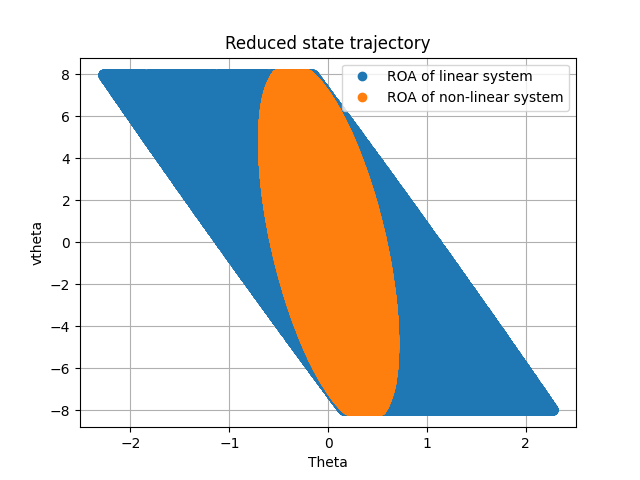
\includegraphics[width=0.65\textwidth]{ROA_comparison}
    \caption{It is intuitive to think that the ROA decreases linearly with the number of constraints set to the LMI}
\end{figure}

\subsection*{Extension to dynamic ETM}
To further extend the problem the LMI formulation has been changed. A dynamic threshold on the ETM mechanism as been added and some matrices have been changed to account for the possible reference to include in the integrator dynamics. 
The same mechanism introduced in (\ref{ETM-mechanism}) and (\ref{eta-dyn}) has been used. 

Now each layer will have its own dynamical threshold:

\begin{align*}
  \eta_i^{+} &= (\rho_{i} + \lambda_{i}) \eta_i - \psi \\
  \eta^{+} &= \bmx{
    \eta_1^{+} \\
    \vdots \\
    \eta_l^{+}
  } = \left( \bmx{
    \rho_1 & 0 & \dots & 0\\
    0 & \rho_2 & \dots & 0\\
    \vdots & \vdots & \ddots & \vdots\\
    0 & 0 & \dots & \rho_l
  } + \bmx{
    \lambda_1 & 0 & \dots & 0\\
    0 & \lambda_2 & \dots & 0\\
    \vdots & \vdots & \ddots & \vdots\\
    0 & 0 & \dots & \lambda_l
  }\right) \bmx{
    \eta_1 \\
    \vdots \\
    \eta_l
  } - \bmx{
    \psi_1 \\
    \vdots \\
    \psi_l
  } = \\
  &= \left( R + L \right) \eta - \psi
\end{align*}

I define the vector $\one \in \RR^{n_{x}} = \bmx{1 & \dots & 1}\tr$

And the Lyapunov function is now defined as $V = \tilde{x}\tr P \tilde{x} + He \left\{ \one\tr \eta \right\}$.
The ETM mechanism for the $i$-th layer now includes the sector conditions for the activation functions and a contribution relative to the integrator state:

$$
  \tilde{\psi}\tr T \left[ G \tilde{x} - \tilde{\nu} + \tilde{\psi} \right] - k\tr \Omega k \geq R \eta
$$

With $k$ being the integrator $C x - r$ and $\Omega$ being a positive definite diagonal matrix. The dynamic of the integrator can now be possibly expressed as $z^{+} = z + k = z + C x - r$. There is a particular property in this configuration being the first element of $C \tilde{x} = C x - r$. This is useful because it doesn't require us to add another term $r$ in this case to the extended vector and still regroup everything with respect to $\left[ \tilde{x}, \tilde{\psi}, \tilde{\phi} \right]\tr$.
The dynamic of the system can be expressed by:

$$
  x^{+} = A x + B u + C \phi + D r \to \tilde{x}^{+} = A \tilde{x} + B \tilde{\psi} + C \tilde{\phi} + D r - D r = A \tilde{x} + B \tilde{\psi} + C \tilde{\phi}
$$

I rewrite the sector conditions in a more compact way expressing:

\begin{align*}
  \Phi &= \bmx{
    \tilde{\psi}_{1}\tr T_{1} [G_{1} \tilde{x} - \tilde{\nu}_{1} + \tilde{\psi}_{1}] - k\tr \Omega_{1} k  & \cdots & 0 \\
    \vdots & \ddots & \vdots \\
    0 & \cdots & \tilde{\psi}_{l}\tr T_{l} [G_{l} \tilde{x} - \tilde{\nu}_{l} + \tilde{\psi}_{l}] - k\tr \Omega_{l} k
  } = \\
  &= \bmx{
    \tilde{x} \\
    \tilde{\psi} \\
    \tilde{\phi}
  }\tr \bmx{
    -C_{k}\tr \Omega C_{k} & 0 & 0 & 0 & 0 \\
    TG & -T & T & 0 & 0 \\
    0 & 0 & 0 & 0 & 0 
  } \bmx{
    \tilde{x} \\
    \tilde{\psi} \\
    \tilde{\nu} \\
    \tilde{\phi} \\
  } = \\
  &= \bmx{
    \tilde{x} \\
    \tilde{\psi} \\
    \tilde{\phi}
  }\tr \bmx{
    -C_{k}\tr \Omega C_{k} & 0 & 0 & 0 & 0 \\
    TG & -T & T & 0 & 0 \\
    0 & 0 & 0 & 0 & 0 
  } \bmx{
    \Id & 0 & 0 \\
    R N_{\nu x} & \Id - R & 0 \\
    0 & \Id & 0 \\
    0 & 0 & \Id 
  } \bmx{
    \tilde{x} \\
    \tilde{\psi} \\
    \tilde{\phi}
  }
\end{align*}

With $C_{k} \in \RR^{n_{\phi} \times n_{x}} = \bmx{
  1 & 0 & 0 \\
  \vdots & \vdots & \vdots \\
  1 & 0 & 0 
}$ selected to extract just the $\theta$ parameter from the state $x$.
$\eta^{+}$ can be rewritten as: $\eta^{+} = (R + L) \eta - \Phi \one$
With this condensed notation I proceed to discuss the sign of the increment of the Lyapunov function $\Delta V$ with respect to equation. \ref{matricione}:

\begin{align*}
  \Delta V &= (\tilde{x}^{+})\tr P (\tilde{x}^{+}) + He\left\{ \one\tr \eta^{+} \right\} - \tilde{x}\tr P \tilde{x} - He\left\{ \one\tr \eta \right\} =\\
  &= \left( A \tilde{x} + B \tilde{u} + C \tilde{\phi} \right)\tr P \left( A \tilde{x} + B \tilde{u} + C \tilde{\phi} \right) - \tilde{x}\tr P \tilde{x} + He\left\{ \one\tr \left(   \left( R + L \right)\eta - \Phi \one - \eta  \right) \right\} = \\
  &= \bmx{
    \tilde{x}\\
    \tilde{\psi}\\
    \tilde{\phi}
  }\tr \bmx{
    \bar{A}\tr P \bar{A} - P & \bar{A}\tr P \bar{B} & \bar{A}\tr P C \\
    \bar{B}\tr P \bar{A} & \bar{B}\tr P \bar{B} & \bar{B}\tr P C \\
    C\tr P \bar{A} & C\tr P \bar{B} & C\tr P C
  } \bmx{
    \tilde{x}\\
    \tilde{\psi}\\
    \tilde{\phi}
  } + He\left\{ \one\tr \left( \left( R + L - I \right) \eta - \Phi \one \right) \right\} =
\end{align*}

I can synthesize the ETM condition rewriting something like: $\Phi \one \geq R \eta$ that holds element-wise. I can then exploit $\eta \leq R^{-1} \Phi \one$ and plug it in $\Delta V$ to get rid of $\eta$:

\begin{align*}
  \Delta V &= \bmx{
    \tilde{x}\\
    \tilde{\psi}\\
    \tilde{\phi}
  }\tr M \bmx{
    \tilde{x}\\
    \tilde{\psi}\\
    \tilde{\phi}
  } + He\left\{ \one\tr \left( \left( R + L - I \right) R^{-1} \Phi \one - \Phi \one \right) \right\} = \\
  &= \bmx{
    \tilde{x}\\
    \tilde{\psi}\\
    \tilde{\phi}
  }\tr M \bmx{
    \tilde{x}\\
    \tilde{\psi}\\
    \tilde{\phi}
  } + He\left\{ \one\tr \left( L - I \right) R^{-1} \Phi \one \right\} < 0
\end{align*}

Calling now $ \Gamma = (L - I) R^{-1} $ and regrouping everything with respect to the augmented vector I can rewrite:

\begin{align*}
  \Delta V &= \bmx{
    \tilde{x}\\
    \tilde{\psi}\\
    \tilde{\phi}
  }\tr M \bmx{
    \tilde{x}\\
    \tilde{\psi}\\
    \tilde{\phi}
  } - \bmx{
    \tilde{x}\\
    \tilde{\psi}\\
    \tilde{\phi}
  }\tr \bmx{
    -C_{k}\tr \Gamma \Omega C_{k} & 0 & 0 & 0 & 0 \\
    \Gamma T G & - \Gamma T & \Gamma T & 0 & 0 \\
    0 & 0 & 0 & 0 & 0
  } \bmx{
    Id & 0 & 0 \\
    R N_{\nu x} & Id - R & 0 \\
    0 & Id & 0\\
    0 & 0 & Id
  } \bmx{
    \tilde{x}\\
    \tilde{\psi}\\
    \tilde{\phi}
  } = \\
  &= \bmx{
    \tilde{x}\\
    \tilde{\psi}\\
    \tilde{\phi}
  }\tr \left( M - M_{\pi} R_{\pi} - R_{\pi}\tr M_{\pi}\tr \right) \bmx{
    \tilde{x}\\
    \tilde{\psi}\\
    \tilde{\phi}
  }
\end{align*}

Finally, adding the sector conditions for the non-linearity $\phi$ like in equation. \ref{V-condition} I can impose the negative definiteness of the Lyapunov function derivative:

\begin{equation}
  \Delta V \leq \bmx{
    \tilde{x}\\
    \tilde{\psi}\\
    \tilde{\phi}
  }\tr \left( 
    M - M_{\pi} R_{\pi} - R_{\pi}\tr M_{\pi}\tr - R_{q}\tr \bmx{
      0 & -1 \\
      -1 & -2
    } R_{q}
   \right) \bmx{
    \tilde{x}\\
    \tilde{\psi}\\
    \tilde{\phi}
   }
\end{equation}

Given the local validity of the sector conditions for the activation functions it's necessary to add some ellipsoid conditions to the Lyapunov function. I want $\tilde{x}\tr \alpha P \tilde{x} \leq 1$, from the sector condition definition, see set $\cS$ in \cite{css-extended} I have:

$$
  \cS = \left\{ x(k) \in \RR^{n_{p}} : -\bar{\nu} - \nu_* \leq G (x(k) - x_*) \leq \bar{\nu} - \nu_* \right\}
$$

Since $\nu_* = 0$ the condition directly translates into $|G \tilde{x}| \leq \bar{\nu} \to (G \tilde{x})\tr (G \tilde{x}) \leq \bar{\nu}^2 \to \tilde{x}\tr \frac{G\tr G}{\bar{\nu}^{2}} \tilde{x} \leq 1$ I want this condition to be included in the ellipsoid defined by $\cE(P, x_*) = \left\{ x \in \RR^{n_{F}}: \tilde{x}\tr \gamma P \tilde{x} \leq 1 \right\}$

\begin{multline*}
  \tilde{x}\tr \frac{G\tr G}{\bar{\nu}^{2}} \tilde{x} \leq \tilde{x}\tr \gamma P \tilde{x} \leq 1 \to \frac{G\tr G}{\bar{\nu}^{2}} \leq \gamma P \leq 1 \to \gamma P - \frac{G\tr G}{\bar{\nu}^{2}} \geq 0\\
  0
\end{multline*}

It is now possible to apply Schur's complement, dividing everything by $\gamma$:

\begin{equation}
  P - \frac{G\tr G}{\gamma \bar{\nu}^{2}} \geq 0 \to \bmx{P & G\tr\\ G & \gamma \bar{\nu}^{2}} \geq 0
\end{equation}

Now by pre and post multiplying by $\bmx{\Id & 0\\ 0 & T}$:

\begin{equation}\label{ellipsoid}
  \bmx{P & G\tr T\\
  TG & \gamma \bar{\nu}^{2} T^{2}} \geq 0
\end{equation}

Equation \ref{ellipsoid} is the last LMI condition to add. The problem arises due to the bilinear term $TG$. A new change of variable is introduced: $Z \triangleq TG$. Doing so we deal with the bilinear term that appears here and in $M_{\pi}$. We still have to deal with the bilinear term $T^{2}$. Following the same approach as in \cite{css-extended} I exploit the inequality:

$$
  \left[ \alpha \bar{\nu}^{-2} - T \right] \bar{\nu}^{2}\left[ \alpha \bar{\nu}^{-2} - T \right] \geq 0 \to \alpha^{2} \bar{\nu}^{-2} - 2 \alpha T + \bar{\nu}^{2} T^{2} \geq 0 \to \bar{\nu}^{2} T^{2} \geq 2 \alpha T - \alpha^{2} \bar{\nu}^{-2}
$$

I can rewrite the ellipsoid condition as putting $\gamma = 1$

$$
  \bmx{P & Z\tr\\
  Z & \bar{\nu}^{2} T^{2}} \geq \bmx{
    P & Z\tr\\
    Z & 2 \alpha T - \alpha^{2} \bar{\nu}^{-2}
  } \geq 0
$$

More precisely a condition like the previous has to be imposed for each activation function in the network. Then we have to discuss the value of $\alpha$: the unitary value works but results to give conservative results. To find the optimal value a golden-section search algorithm can be used since the problem to address can be expressed as an unimodal function defined on a given interval, it has the advantage to reduce the search interval by a constant factor at each step.

\begin{enumerate}
    \item \textbf{Define the Interval and the Golden Ratio:} \\
    Let $[a = 1, b = 0]$ be the initial interval containing the values for which the LMI is feasible. Defining the golden ratio $\varphi$ as:
    $$
    \varphi = \frac{1 + \sqrt{5}}{2}
    $$
    
    \item \textbf{Set Initial Interior Points:} \\
    Calculate two interior points $ \alpha_1 $ and $ \alpha_2 $ within $[a, b]$ such that:
    $$
    x_1 = b - \frac{b - a}{\varphi}, \quad x_2 = a + \frac{b - a}{\varphi}.
    $$
    
    \item \textbf{Solve the LMI:} \\
    Solve the LMI and store the value of the maximum eigenvalue of the $P$ matrix: $ \lambda_1, \lambda_2 $.
    
    \item \textbf{Narrow the Interval:} \\
    Based on the values $ \lambda_1, \lambda_2$, update the interval $[a, b]$ as follows:
    \begin{itemize}
        \item If $ \lambda_1 < \lambda_2 $, then the minimum is in the interval $[a, x_2]$. Set $ b = x_2 $.
        \item If $ \lambda_2 < \lambda_1 $, then the minimum is in the interval $[x_1, b]$. Set $ a = x_1 $.
    \end{itemize}
    
    \item \textbf{Repeat the Process:} \\
    Recalculate $ x_1 $ and $ x_2 $ within the new interval $[a, b]$ and repeat steps 3 and 4. At each iteration, the interval is reduced by a factor of the golden ratio, retaining only the portion containing the minimum.
    
    \item \textbf{Convergence:} \\
    Continue until the length of the interval $[a, b]$ is less than a chosen tolerance level, $\epsilon$. At this point, any $\alpha$ value within the interval can be considered to give the biggest Region of attraction estimate.
\end{enumerate}

After solving the LMI, even though the solution is found the ROA is still incredibly small. In addition to that the LMI finds a solution such that $\Omega$ has every item close to 0, this means that the "help" we want to give the ETM to trigger less is not helpful to the LMI problem and is therefore ignored. 

Since no other tweaks on the LMI formulation seems to be possible the next approach will be using the currently deep learning trained network and re-train it with RL by projecting a solution of the LMI in each training step to enlarge as much as possible the starting ROA. 

\section*{Retraining of NN with RL to enlarge the ROA}
The main problem now is to design an efficient cost function to enlarge the ROA. After a first brainstorm the ideas are:
\begin{itemize}
  \item Give as a cost $ln(1/\bar{\lambda})$ with $\bar{\lambda}$ the maximum eigenvalue of last $P$. 
  \item Use $\Delta V$ when it's negative as a cost. Like a $\texttt{relu}(\Delta V)$.
\end{itemize}

The problem under examination is now the simpler non-linear pendulum without integrator in the state. A new starting network has been trained with deep neural network based on a linear LQR controller. Now the two approaches listed before will be followed:

\begin{itemize}
  \item The first approach sees the treatment of the environment as the NN itself. The action will be a list of increments to add to each element of the weights and the biases. The starting point will be the previously trained network. A step is the creation of the new weights and biases and solve the LMI for them. The cost will be continuous and proportional to the area of the ROA found. If infeasible the cost will be $0$. The length of one episode will be decided a priori. If we have a better solution that gives a bigger ROA then the weights will be stored but not updated. They will be updated only on reset and if we have an increment in the ROA's area that is big enough. Another aspect to take into account is the size of the training NN. The action will be a vector of $\simeq 2100$ elements.

  \textbf{This method was discarded because of the big dimension of the action. Several attempts were executed but with no good results.}

  \item This SEEMS easier to implement. A rollout of the system will be done and the $\Delta V$ of the rollout will be computed with respect to the last $P$ found, it will then be used as a cost. The architecture of the NN should be the same as the one trained with deep learning and should accept as a starting point the previously trained weights and biases. At each reset a LMI will be solved, if it leads to a bigger ROA then the $P$ matrix to which we refer to improve will be updated.
\end{itemize}

Last method resulted to be the efficient one. It was hard to set up correctly the environment to make it compliant with \texttt{stable\_baselines3}, in particular the handling of the LMI mid-training and the following update of the current P matrix stored by the environment. 
Rather than a linear method a sequence of different tests has been done to find the best hyperparameters for the training. Initially the results from the \textit{LQR} solution were used as a "warm start" to try and find solutions that led to bigger Region of Attractions. To accomplish so two different reward functions design were alternatively used:

\begin{itemize}
  \item Classical RL reward: $J = -w_{\theta} \theta^2 - w_{v} v^2 - w_{\eta} \eta^2 - w_{u} u^2 + \delta$\\
  Where $\delta$ is a small constant that acts as a constant reward for each step the policy manages to keep the environment "alive". Even if not directly demonstrated using a reward function shaped like this should give results similar in quality to the LQR since both approaches try to minimize the quadratic weight of the state and the control input. 
  \item Custom defined reward: $J = - \Delta V + \frac{\Delta(ROA)}{n_{episode}}$
  
  Here directly passing $\Delta V$ serves to tell the algorithm to penalize every action that leads to a Lyapunov function that is not strictly decreasing. The second term is a bonus that is given to the agent when it manages to enlarge the ROA, since the update of the policy is done at the end of each rollout the bonus is divided by the number of episodes to make the reward small enough to not overshadow the $\Delta V$ term. If the current policy update gives a bigger ROA then the weights are stored and the $\Delta(ROA)$ is instead the overall area of the ROA found, hence giving a bit more reward than cost. Also, the $P$ matrix that is used to compute the reward is updated with the last one found.

  An important aspect that had to be taken into account is the nature of the action give by the RL algorithm being normalized between $-1$ and $1$. To address this peculiarity the LQR solution was found again to be compliant. Given the normalized nature of the action that then get multiplied by the maximum torque appliable by the system I thought to consider it as a saturation applied to the output of the NN and the input of the system. I modified accordingly the LMI by adding an element to the matrices that manage the activation functions sector conditions and another constraint for the ellipsoid condition that now takes the maximum torque as a bound and not the saturation functions value used in the activation function.

  By empirical observations it has been noticed that after a certain amount of rollouts the algorithm stopped to find feasible policy updates. To overcome this problem a new logic has been added: after a certain amount of rollouts without improvements or in the occurrence of an infeasible update the policy would be restored to the best one found so far, the optimizer is also reset and hence the training starts again from the best policy found so far. The good thing about this approach is the fact that the rollout buffer is not emptied hence, even if very slowly, the algorithm can still find better policies in the long term. After many iterations and several runs I ended up with a ROA that is more than 50 times larger in volume than the one found after the deep learning training.
\end{itemize}

\section*{New direction of the research}
Once the ROA has been enlarged the next step is to try and find a direction to present the results found so far. A first idea is to make the paper centered around the ETM implementation. Using the new policy already it shows that it is feasible with dynamic ETM. The behavior is good characterized by a very high update rate of the first layer ($\simeq 100\%$) but the update rate of the last layer, the one responsible for the actual input update to the system, is more than halved stabilizing around $40\%$. Obviously the addition of the ETM mechanism makes the system more conservative since it reduces the Region of Attraction. For this reason we want now to find a way to make the reduction of the ROA preserve some particular directions that are now guaranteed to have more stable states due to the addition of the integrator in the dynamics.

To address this problem Samuele advised to look at some work regarding multi-objective LMIs and to look at previous works of Sophie. Most probably It will be translated into the application of another constraint to the $\Delta V$ sign in the LMI and some change in the objective of the problem definition. 

Ideas to address:
\begin{itemize}
  \item Since the current static ETM matches the minimum feasible ROA we could think of some other ETM mechanism. To be clearer the quadratic constraints of the non-linearities of the activation functions are mandatory and cannot be neglected. Since the static ETM uses the exact same conditions It is clear that the ROA will be the same. 
  \item One possible criteria to try and obtain with an ETM is something regarding the inter-event period and the preferred direction to preserve in ROA shrinking. In particular the direction around $\theta$ since the addition of the integrator in the dynamics makes the system more stable in that direction. Some work of Sophie should have addressed something similar. As regards the inter-event period look at some work of Antoine Girard.
  \item Another possible improvement is changing the quadratic constraints whenever we have some fixed matrices like the one used to address the $sin(\theta) - \theta$ non-linearity. It sees the addition of new variables and constraints to the LMI like seen in the two \textit{k-contraction} papers of Samuele.
  \item The last idea is to try and find a way to implement multiple objectives in the LMI. There are some papers to take idea from like in \cite{multiobjective-1} and \cite{multiobjective-2}.
\end{itemize}

After fixing some error on $x_{*}$ computation solving the following implicit equation:

\begin{align*}
  x^{+} &= A x + B u + C \phi + D r\\
  x_{*} &= A x_{*} + B u_{*} + C \phi(x_{*}) + D r \\
  u_{*} &= N_{ux} x_{*} + N_{u \omega} \omega_{*} + N_{ub} = \\
  &= N_{ux} x_{*} + N_{u \omega} \nu_{*} + N_{ub} = \\
  &= N_{ux} x_{*} + N_{u \omega} \left( \Id - N_{\nu \omega} \right) ^{-1} \left(  N_{\nu x} x_{*} + N_{\nu b}\right) + N_{\nu b} = \\
  &= \left( N_{ux} + N_{u \omega} R N_{\nu x} \right) x_{*} + N_{u \omega} R N_{\nu b} + N_{ub} = R_{\omega} x_{*} + R_{b}\\
  x_{*} &= A x_{*} + B R_{\omega} x_{*} + B R_{b} + C \left( sin(K x_{*}) - K x \right) + D r = \\
  x_{*} &= \left( A + B R_{\omega} - C K \right) x_{*} + B R_{b} + C sin(K x_{*}) + D r
\end{align*}

Hence, the implicit equation to solve is:

\begin{equation}
  \textit{func}(x) = (-I + A + B R_{\omega} - C K) x + B R_{b} + C sin(K x) + D r 
\end{equation}

With $K = \bmx{1 & 0 & 0}$
 
The issue I wanted to solve was the continuous update and event triggering even after the system has reached the equilibrium. The equilibrium reach was confirmed by inspecting the behavior of the system, it has been shown a Lyapunov function that tends to 0 (order of $1e-30$) and a norm of $\tilde{x} = x - x_{*}$ that tends to 0 (order of $1e-6$) after just 300 steps. The control input also tends to $u_{*}$ faster than the state but slower than the Lyapunov.
The intuition was to add some threshold on the magnitude of the actors of the ETM, since the ETM mechanism defined by $
  \Psi \geq \rho \eta $ triggers around equilibrium for very small values of $\Psi$ (around $1e-30$) by adding a random threshold small enough, even if it was not yet implemented in the LMI, an improvement on the update rate has been noticed. However, it didn't eliminate the behavior we wanted to avoid being the non-necessary updates once the equilibrium has been reached. An increment on the update rate has been observed until the threshold was not big enough to mess up all the system and ETM mechanism.

  To continue addressing the problem I will look into the \textit{"Stubborn State Observers"} topic first introduced by Luca. See \cite{stubborn-1}, \cite{stubborn-2} and \cite{stubborn-3}.

  \subsection*{Finsler's Lemma workaround}
  
  A way to try and solve the problem was to use a different matrix for the ETM. For the $i^{th}$ layer it was used the following matrix so far:

  $$    
    \bmx{
      \tilde{x}\\
      \tilde{\psi_{i}}\\
      \tilde{\nu_{i}}
    }\tr
    \Omega_{i}
    \bmx{
      \tilde{x}\\
      \tilde{\psi_{i}}\\
      \tilde{\nu_{i}}
    } = \bmx{
      \tilde{x}\\
      \tilde{\psi_{i}}\\
      \tilde{\nu_{i}}
    }\tr
    \bmx{
      0 & 0 & 0\\
      T_{i} G_{i} & T_{i} & -T_{i}\\
      0 & 0 & 0 
    }
    \bmx{
      \tilde{x}\\
      \tilde{\psi_{i}}\\
      \tilde{\nu_{i}}
    }
  $$

  With $TG = Z$ to address the bilinear term. Due to the sparseness of $\Omega$ we want to find a denser matrix $X$ that approximates $\Omega$ and is compliant with the Finsler's Lemma. It can be done by adding the following constraint in the LMI:

  $$
  \Omega = \bmx{
    \begin{array}{ccc|ccc|ccc}
      0 & 0 & 0 & 0 & 0 & 0 & 0 & 0 & 0\\
      Z_{1} & T_{1} & -T_{1} & 0 & 0 & 0 & 0 & 0 & 0\\
      0 & 0 & 0 & 0 & 0 & 0 & 0 & 0 & 0\\
      \hline
      0 & 0 & 0 & 0 & 0 & 0 & 0 & 0 & 0\\
      0 & 0 & 0 & Z_{2} & T_{2} & -T_{2} & 0 & 0 & 0\\
      0 & 0 & 0 & 0 & 0 & 0 & 0 & 0 & 0\\
      \hline
      0 & 0 & 0 & 0 & 0 & 0 & 0 & 0 & 0\\
      0 & 0 & 0 & 0 & 0 & 0 & Z_{3} & T_{3} & -T_{3}\\
      0 & 0 & 0 & 0 & 0 & 0 & 0 & 0 & 0\\
    \end{array}
  }
$$

$$
  X = \bmx{
    \begin{array}{c|c|c}
      X_{1} & 0 & 0\\
      \hline
      0 & X_{2} & 0\\
      \hline
      0 & 0 & X_{3}
    \end{array}
  }
$$
  
$$
R_{\xi}\tr He\left\{ X - \Omega \right\} R_{\xi} + He \left\{  \pmx{N_{1} \\ N_{2} \\ N_{3}} \pmx{R N_{\nu x} & \Id - R & -\Id} \right\} \leq 0
$$

The matrix $R_{\xi}$ orders the vector that should be multiplied by $X$ and $\Omega$:

$$
     \bmx{
      \tilde{x}\\
      \tilde{\psi}\\
      \tilde{\nu}
     } = \bmx{
      \tilde{x}\\
      \tilde{\psi_{1}}\\
      \tilde{\psi_{2}}\\
      \tilde{\psi_{3}}\\
      \tilde{\nu_{1}}\\
      \tilde{\nu_{2}}\\
      \tilde{\nu_{3}}
    } = \bmx{
      \tilde{x}\\
      \tilde{\psi_{1}}\\
      \tilde{\nu_{1}}\\
      \tilde{x}\\
      \tilde{\psi_{2}}\\
      \tilde{\nu_{2}}\\
      \tilde{x}\\
      \tilde{\psi_{3}}\\
      \tilde{\nu_{3}}
    } R_{\xi} = \bmx{
      \tilde{x}\\
      \tilde{\psi_{1}}\\
      \tilde{\nu_{1}}\\
      \tilde{x}\\
      \tilde{\psi_{2}}\\
      \tilde{\nu_{2}}\\
      \tilde{x}\\
      \tilde{\psi_{3}}\\
      \tilde{\nu_{3}}
    } \bmx{
      \Id & 0 & 0 & 0 & 0 & 0 & 0\\
      0 & \Id & 0 & 0 & 0 & 0 & 0\\
      0 & 0 & 0 & 0 & \Id & 0 & 0\\
      0 & 0 & 0 & 0 & 0 & 0 & 0\\
      0 & 0 & \Id & 0 & 0 & 0 & 0\\
      0 & 0 & 0 & 0 & 0 & \Id & 0\\
      0 & 0 & 0 & 0 & 0 & 0 & 0\\
      0 & 0 & 0 & \Id & 0 & 0 & 0\\
      0 & 0 & 0 & 0 & 0 & 0 & \Id
    } 
$$

With this condensed notation I proceed to discuss the sign of the increment of the Lyapunov function $\Delta V$. I start by plugging the ETM condition, further considerations on the proper sector conditions will be done later. Now the matrix $X$ is used instead of $\Omega$:

\begin{align*}
  \Delta V &= (\tilde{x}^{+})\tr P (\tilde{x}^{+}) + He\left\{ \one\tr \eta^{+} \right\} - \tilde{x}\tr P \tilde{x} - He\left\{ \one\tr \eta \right\} =\\
  &= \left( A \tilde{x} + B \tilde{u} + C \tilde{\phi} \right)\tr P \left( A \tilde{x} + B \tilde{u} + C \tilde{\phi} \right) - \tilde{x}\tr P \tilde{x} + He\left\{ \one\tr \left(   \left( R + L \right)\eta - X \one - \eta  \right) \right\} = \\
  &= \bmx{
    \tilde{x}\\
    \tilde{\psi}\\
    \tilde{\phi}
  }\tr \bmx{
    \bar{A}\tr P \bar{A} - P & \bar{A}\tr P \bar{B} & \bar{A}\tr P C \\
    \bar{B}\tr P \bar{A} & \bar{B}\tr P \bar{B} & \bar{B}\tr P C \\
    C\tr P \bar{A} & C\tr P \bar{B} & C\tr P C
  } \bmx{
    \tilde{x}\\
    \tilde{\psi}\\
    \tilde{\phi}
  } + He\left\{ \one\tr \left( \left( R + L - I \right) \eta - X \one \right) \right\} =
\end{align*}

I can synthesize the ETM condition rewriting something like: $X \one \geq R \eta$ that holds element-wise. I can then exploit $\eta \leq R^{-1} X \one$ and plug it in $\Delta V$ to get rid of $\eta$:

\begin{align*}
  \Delta V &= \bmx{
    \tilde{x}\\
    \tilde{\psi}\\
    \tilde{\phi}
  }\tr M \bmx{
    \tilde{x}\\
    \tilde{\psi}\\
    \tilde{\phi}
  } + He\left\{ \one\tr \left( \left( R + L - I \right) R^{-1} X \one - X \one \right) \right\} = \\
  &= \bmx{
    \tilde{x}\\
    \tilde{\psi}\\
    \tilde{\phi}
  }\tr M \bmx{
    \tilde{x}\\
    \tilde{\psi}\\
    \tilde{\phi}
  } + He\left\{ \one\tr \left( L - I \right) R^{-1} X \one \right\} < 0
\end{align*}

Calling now $ \Gamma = (L - I) R^{-1} $ and regrouping everything with respect to the augmented vector I can rewrite:

\begin{align*}
  \Delta V &= \bmx{
    \tilde{x}\\
    \tilde{\psi}\\
    \tilde{\phi}
  }\tr M \bmx{
    \tilde{x}\\
    \tilde{\psi}\\
    \tilde{\phi}
  } + \bmx{
    \tilde{x}\\
    \tilde{\psi}\\
    \tilde{\phi}
  }\tr R_{\nu}\tr \bar{R_{\xi}}\tr 
  He \left\{ \Gamma \bar{X}  \right\} \bar{R_{\xi}} R_{\nu} \bmx{
    \tilde{x}\\
    \tilde{\psi}\\
    \tilde{\phi}
  }
\end{align*}

The matrix $\bar{R_{\xi}}$ now takes into account the non-linearity $\tilde{\phi}$, the matrix $R_{\nu}$ takes care of $\tilde{\nu}$ 

$$
  \bar{R_{\xi}} = \bmx{
  \begin{array}{c | c}
    R_{\xi} & 0\\
    \hline
    0 & \Id
  \end{array}
  }; R_{\nu} = \bmx{
    \Id & 0 & 0\\
    0 & \Id & 0\\
    R N_{\nu x} & \Id - R & 0\\
    0 & 0 & \Id
  }
$$

Now the previously seen sector conditions for the sin non linearities can be added in the same way as before. 

\textbf{SHOULD I ADD SECTOR CONDITIONS FOR ETM OR ARE THEY ALREADY TAKEN INTO ACCOUNT INSIDE THE FINSLER CONDITIONS?}

\pagebreak
\emergencystretch=2em % To account for hbox overflow warning
\printbibliography

\end{document}